% ============================================================
%  Kindred Careers — Graduation Project Documentation
%  Chapters 5, 6 & 7  (Completion Volume)
%
%  Institution  : Ahram Canadian University
%  Supervisor   : Dr. Dieaa Ibrahim
%  Academic Year: 2025–2026
%
%  USAGE:
%    Compile with pdflatex (twice for cross-references):
%      pdflatex chapters_5_6_7.tex
%      pdflatex chapters_5_6_7.tex
%
%  NOTE: Replace every \placeholder{...} tag with the actual
%  figure/screenshot before final submission.
% ============================================================

% ─────────────────────────────────────────────────────────────
%  PREAMBLE
% ─────────────────────────────────────────────────────────────
\documentclass[12pt, a4paper, oneside]{report}

% --- Core Typography & Encoding ---
\usepackage[T1]{fontenc}
\usepackage[utf8]{inputenc}
\usepackage{lmodern}                    % Scalable Computer Modern font
\usepackage{microtype}                  % Subtle typographic improvements

% --- Page Geometry ---
\usepackage[
  top=2.5cm,
  bottom=2.5cm,
  left=3.0cm,
  right=2.5cm,
  headheight=15pt
]{geometry}

% --- Graphics & Figures ---
\usepackage{graphicx}                   % \includegraphics
\usepackage{float}                      % [H] float placement
\usepackage{caption}                    % Custom caption styling
\usepackage{subcaption}                 % Side-by-side figures
\usepackage{xcolor}                     % Colour support
\usepackage{tikz}                       % Inline diagrams / placeholder boxes
\usepackage[most]{tcolorbox}            % Fancy coloured boxes

% --- Tables ---
\usepackage{booktabs}                   % \toprule, \midrule, \bottomrule
\usepackage{tabularx}                   % Auto-width table columns
\usepackage{longtable}                  % Multi-page tables
\usepackage{array}                      % Extended column definitions
\usepackage{multirow}                   % Row-spanning table cells

% --- Code Listings ---
\usepackage{listings}                   % Source-code blocks
\usepackage{inconsolata}                % Monospace font for code

% --- Maths ---
\usepackage{amsmath}
\usepackage{amssymb}

% --- Lists & Enumeration ---
\usepackage{enumitem}

% --- Headers, Footers & Chapter Titles ---
\usepackage{fancyhdr}
\usepackage[explicit]{titlesec}
\usepackage{titletoc}

% --- Hyperlinks (must be near last) ---
\usepackage{hyperref}
\hypersetup{
  colorlinks  = true,
  linkcolor   = black,
  citecolor   = black,
  urlcolor    = blue,
  bookmarks   = true,
  pdfauthor   = {Omier Sameh et al.},
  pdftitle    = {Kindred Careers -- Chapters 5-7},
  pdfsubject  = {Graduation Project Documentation},
  pdfkeywords = {Flutter, FastAPI, RAG, ChromaDB, Job Matching, AI}
}

% --- References ---
\usepackage[numbers, sort&compress]{natbib}
\usepackage{url}

% ─────────────────────────────────────────────────────────────
%  COLOUR PALETTE  (matches university template dark-blue tone)
% ─────────────────────────────────────────────────────────────
\definecolor{kindredblue}{RGB}{30, 58, 138}     % Deep navy
\definecolor{kindredgold}{RGB}{180, 130, 30}    % Warm gold accent
\definecolor{lightgray}{RGB}{245, 245, 245}
\definecolor{codebg}{RGB}{250, 250, 250}
\definecolor{coderule}{RGB}{200, 200, 200}

% ─────────────────────────────────────────────────────────────
%  CHAPTER & SECTION STYLE
% ─────────────────────────────────────────────────────────────
\titleformat{\chapter}[block]
  {\normalfont\LARGE\bfseries\color{kindredblue}}
  {CHAPTER \thechapter}{1em}{#1}
  [\vspace{0.4ex}{\color{kindredgold}\titlerule[1.5pt]}]

\titleformat{\section}
  {\normalfont\large\bfseries\color{kindredblue}}
  {\thesection}{0.8em}{#1}

\titleformat{\subsection}
  {\normalfont\normalsize\bfseries}
  {\thesubsection}{0.8em}{#1}

\titleformat{\subsubsection}
  {\normalfont\normalsize\itshape}
  {\thesubsubsection}{0.8em}{#1}

\titlespacing*{\chapter}{0pt}{0pt}{20pt}
\titlespacing*{\section}{0pt}{12pt}{6pt}
\titlespacing*{\subsection}{0pt}{10pt}{4pt}

% ─────────────────────────────────────────────────────────────
%  PAGE STYLE
% ─────────────────────────────────────────────────────────────
\pagestyle{fancy}
\fancyhf{}
\fancyhead[L]{\small\nouppercase{\leftmark}}
\fancyhead[R]{\small Kindred Careers}
\fancyfoot[C]{\small Page \textbar\ \thepage}
\renewcommand{\headrulewidth}{0.5pt}
\renewcommand{\footrulewidth}{0.5pt}

% ─────────────────────────────────────────────────────────────
%  CODE LISTING STYLE
% ─────────────────────────────────────────────────────────────
\lstdefinestyle{kindredcode}{
  backgroundcolor = \color{codebg},
  basicstyle      = \small\ttfamily,
  keywordstyle    = \bfseries\color{kindredblue},
  commentstyle    = \itshape\color{gray},
  stringstyle     = \color{kindredgold},
  breaklines      = true,
  breakatwhitespace = true,
  frame           = single,
  rulecolor       = \color{coderule},
  numbers         = left,
  numberstyle     = \tiny\color{gray},
  numbersep       = 8pt,
  tabsize         = 4,
  showstringspaces = false,
  captionpos      = b,
}
\lstset{style=kindredcode}

% New languages
\lstdefinelanguage{Dart}{
  keywords = {var, final, const, void, return, class, extends, implements,
              import, export, null, true, false, new, this, super, async,
              await, Future, List, Map, String, int, double, bool, if, else,
              for, while, do, switch, case, break, continue, try, catch,
              throw, abstract, static, dynamic, required, late},
  morecomment  = [l]{//},
  morecomment  = [s]{/*}{*/},
  morestring   = [b]",
  morestring   = [b]',
}

% ─────────────────────────────────────────────────────────────
%  PLACEHOLDER HELPER — draws a labelled grey box
%  Usage: \placeholder{Figure 5.1 — Home Screen screenshot}
% ─────────────────────────────────────────────────────────────
\newcommand{\placeholder}[1]{%
  \begin{tcolorbox}[
    colback  = lightgray,
    colframe = coderule,
    fontupper= \small\ttfamily\color{gray},
    halign   = center,
    valign   = center,
    height   = 6cm,
    sharp corners
  ]
    [IMAGE PLACEHOLDER]\\[4pt]#1
  \end{tcolorbox}%
}

% ─────────────────────────────────────────────────────────────
%  CHAPTER COUNTER — continue numbering from Chapter 4
% ─────────────────────────────────────────────────────────────
\setcounter{chapter}{4}   % Next \chapter increments to 5

% ─────────────────────────────────────────────────────────────
%  DOCUMENT BEGIN
% ─────────────────────────────────────────────────────────────
\begin{document}

% ─────────────────────────────────────────────────────────────
%  ██████████████████  CHAPTER 5  ██████████████████████████
% ─────────────────────────────────────────────────────────────
\chapter{Implementation and Results}

This chapter details the practical realisation of the Kindred Careers system. It covers the
end-to-end software architecture that bridges the Flutter mobile client with the FastAPI
backend, presents the key user-interface screens that embody the project's UX vision, and
provides a thorough walkthrough of every core backend service — from vector-based job retrieval
to AI-powered CV generation.

% ─────────────────────────────────────────────────────────────
\section{Software Architecture}
\label{sec:software-architecture}
% ─────────────────────────────────────────────────────────────

Kindred Careers follows a \textbf{client–server architecture} with a clear separation of
concerns across three tiers:

\begin{enumerate}[label=\textbf{\arabic*.}, leftmargin=*, itemsep=4pt]
  \item \textbf{Presentation Tier} — A Flutter mobile application (Android and iOS) that handles
        all user interactions, renders job cards, and manages local session state.
  \item \textbf{Application Tier} — A FastAPI (Python 3.11) REST backend deployed via
        Uvicorn, responsible for job ingestion, profile embedding, vector-similarity search,
        and AI-driven CV generation.
  \item \textbf{Data Tier} — A dual-database layer comprising:
        \begin{itemize}[itemsep=2pt]
          \item \textbf{ChromaDB} — a locally-persisted vector database that stores 384-dimensional
                job embeddings produced by the \texttt{sentence-transformers/all-MiniLM-L6-v2} model.
          \item \textbf{SQLite (\texttt{swipes.db})} — a lightweight relational store that maintains
                per-user swipe history for stateful exclusion filtering.
          \item \textbf{Firebase Firestore} — cloud-hosted NoSQL database used to persist user
                profiles, authentication tokens, and career-path data.
        \end{itemize}
\end{enumerate}

\noindent The high-level data-flow is illustrated in Figure~\ref{fig:arch-overview}:

\begin{figure}[H]
  \centering
  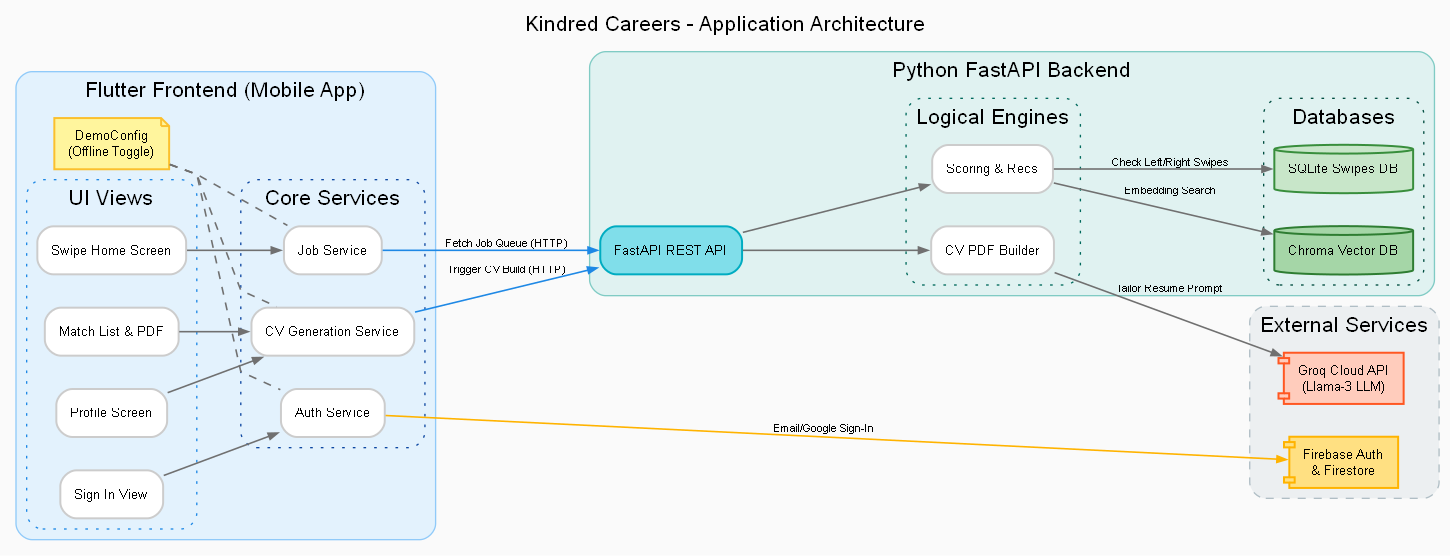
\includegraphics[width=\textwidth]{architecture.pdf}
  \caption{High-level software architecture of Kindred Careers.}
  \label{fig:arch-overview}
\end{figure}

\subsection*{Technology Stack Summary}

\begin{table}[H]
  \centering
  \caption{Technology stack used in Kindred Careers.}
  \label{tab:tech-stack}
  \renewcommand{\arraystretch}{1.35}
  \begin{tabularx}{\textwidth}{@{} l l X @{}}
    \toprule
    \textbf{Layer}       & \textbf{Technology}              & \textbf{Role} \\
    \midrule
    Mobile Frontend      & Flutter 3 / Dart 3               & Cross-platform UI, state management \\
    Backend Framework    & FastAPI 0.115                    & RESTful API server, background tasks \\
    AI / LLM             & Groq API (LLaMA 3 70B)           & CV generation, job summarisation \\
    Embedding Model      & \texttt{all-MiniLM-L6-v2}        & 384-dim semantic job embeddings \\
    Vector Database      & ChromaDB 0.5                     & Similarity search for job matching \\
    Swipe Persistence    & SQLite (\texttt{swipes.db})       & Per-user swipe-exclusion tracking \\
    Auth / Cloud DB      & Firebase Auth + Firestore         & User authentication, profile storage \\
    Web Scraping         & Camoufox + BeautifulSoup4        & Real-time job scraping (Wuzzuf) \\
    PDF Generation       & ReportLab 4                      & ATS-optimised CV export \\
    Containerisation     & Docker                           & Deployment and environment isolation \\
    \bottomrule
  \end{tabularx}
\end{table}

\subsection*{RAG Pipeline Overview}

The Retrieval-Augmented Generation (RAG) pipeline constitutes the intellectual core of Kindred
Careers. It operates in three stages:

\begin{description}[leftmargin=2cm, style=nextline, itemsep=6pt]
  \item[Stage 1 — Ingest]
        The background worker (\texttt{worker.py}) scrapes up to 60 job listings per run from
        Wuzzuf using Camoufox. Each listing is summarised into concise bullet points by the Groq
        LLM (\texttt{job\_summarizer.py}) and then embedded into a 384-dimensional vector via the
        \texttt{all-MiniLM-L6-v2} Sentence Transformer. The result is upserted into ChromaDB using
        a deterministic stable ID (\texttt{job\_\{MD5(title|company)\}}) to prevent duplication
        across scrape runs.

  \item[Stage 2 — Retrieve]
        When the Flutter client calls \texttt{POST /api/jobs/feed}, the backend:
        (a) fetches all job IDs the user has already swiped from \texttt{swipes.db};
        (b) merges them with any client-side \texttt{exclude\_ids};
        (c) embeds the user profile using the same Sentence Transformer;
        (d) runs a cosine-similarity query in ChromaDB against only the unviewed subset.
        The final ranking combines 65\% match score with 35\% recency factor
        ($\text{score} = 0.65 \cdot \text{cosine} + 0.35 \cdot e^{-0.1 \cdot \text{age}}$).

  \item[Stage 3 — Generate]
        When the user swipes right, the Flutter client calls \texttt{POST /api/generate-cv}. The
        backend passes the user profile and the full job description to the LLM, which returns a
        structured JSON CV tailored to that specific role. The CV is then rendered as an
        ATS-optimised PDF via ReportLab and streamed back to the client.
\end{description}

% ─────────────────────────────────────────────────────────────
\section{UI of Application}
\label{sec:ui}
% ─────────────────────────────────────────────────────────────

The Kindred Careers user interface was designed around a single guiding principle:
\textbf{zero cognitive load}. At any given moment the user sees exactly one job card. This
binary decision framework — swipe right to apply, swipe left to skip — reduces the
overwhelming nature of traditional job-board list views. The UI was built using Flutter's
widget tree with a custom dark-mode theme (\texttt{app\_theme.dart}) that enforces a
consistent colour palette, typography hierarchy, and animation system throughout the
application.

\subsection{Key Interface Components}
\label{sec:ui-components}

The application is composed of six primary screens and a shared widget library. Each screen is
described below with annotated screenshots.

\subsubsection*{1. Onboarding Screen}

The onboarding flow (\texttt{onboarding\_screen.dart}) greets first-time users with a
full-screen animated splash that communicates the core value proposition of the application.
It consists of three slides: \emph{Discover Jobs}, \emph{Swipe to Match}, and
\emph{Build Your CV}. Users advance through slides with horizontal swipe gestures, providing
an immediate preview of the core interaction model.

\begin{figure}[H]
  \centering
  \placeholder{Figure 5.2 — Onboarding Screen (Slides 1–3)\\Animated value-proposition carousel}
  \caption{Onboarding carousel presented to first-time users.}
  \label{fig:onboarding}
\end{figure}

\subsubsection*{2. Authentication Screen}

The Sign-In screen (\texttt{sign\_in\_screen.dart}) supports two authentication paths:
\begin{itemize}[itemsep=2pt]
  \item \textbf{Email/Password} — validated via Firebase Authentication with built-in
        account-lockout after five consecutive failed attempts.
  \item \textbf{Google Sign-In} — one-tap OAuth2 flow using the \texttt{google\_sign\_in}
        Flutter package.
\end{itemize}

\begin{figure}[H]
  \centering
  \placeholder{Figure 5.3 — Sign In / Register Screen\\Email, password fields and Google OAuth button}
  \caption{Authentication screen with dual sign-in options.}
  \label{fig:signin}
\end{figure}

\subsubsection*{3. Career Questionnaire Screen}

On first login, users are directed to the questionnaire screen
(\texttt{questionnaire\_screen.dart}), a multi-step form that collects:
\begin{itemize}[itemsep=2pt]
  \item Personal details (name, location, phone, bio)
  \item Career fields and preferred work mode (Remote / Hybrid / Onsite)
  \item Skills (chip-based multi-select input)
  \item Work experience (multiple entries with date pickers)
  \item Education (degree, institution, graduation year)
\end{itemize}

This structured data is used to build the \texttt{UserProfile} object serialised on every
API call to the backend for personalised job retrieval and CV generation.

\begin{figure}[H]
  \centering
  \placeholder{Figure 5.4 — Career Questionnaire Screen\\Multi-step profile builder with skill chips}
  \caption{Career questionnaire — step-by-step profile construction.}
  \label{fig:questionnaire}
\end{figure}

\subsubsection*{4. Home Screen — Swipe Feed}

The Home Screen (\texttt{home\_screen.dart}) is the application's primary interface. It
features a tinder-style swipe deck powered by the \texttt{JobRecommendationService} (v2.1 —
Stateful Queue). Key UX details:

\begin{itemize}[itemsep=3pt]
  \item \textbf{Card Stack} — the top card is the active job; cards below provide depth cues.
  \item \textbf{Swipe Gestures} — right-swipe triggers CV generation; left-swipe discards.
  \item \textbf{Match Score Badge} — displays the cosine-similarity percentage prominently.
  \item \textbf{Vibe Tag} — a personality label (e.g.\ ``Fast-paced Startup'') generated
        by the LLM to quickly characterise company culture.
  \item \textbf{Summary Bullets} — three AI-generated bullet points that condense the full
        job description for at-a-glance reading.
  \item \textbf{Stateful Queue Pagination} — a background refresh is triggered automatically
        after every 5 swipes or 60 seconds of active swiping, keeping the feed populated
        without any visible interruption.
\end{itemize}

\begin{figure}[H]
  \centering
  \placeholder{Figure 5.5 — Home Screen: Swipe Feed\\Job card with match score, vibe tag, and bullet summary}
  \caption{Home screen swipe feed with AI-enriched job card.}
  \label{fig:homescreen}
\end{figure}

\subsubsection*{5. Matched Jobs Screen}

The Matched Jobs screen (\texttt{matched\_jobs\_screen.dart}) serves as the user's job
application dashboard. When a user swipes right on a job, the system:
\begin{enumerate}[label=\arabic*., itemsep=2pt]
  \item Persists the swipe to Firebase Firestore.
  \item Calls \texttt{POST /api/generate-cv} to produce a tailored CV JSON.
  \item Displays a loading indicator while the LLM processes.
  \item Renders the generated CV in a structured preview card.
  \item Offers the user options to: \emph{Accept}, \emph{Regenerate with Feedback}, or
        \emph{Download as PDF}.
\end{enumerate}

\begin{figure}[H]
  \centering
  \placeholder{Figure 5.6 — Matched Jobs Screen\\Liked job list with AI-generated CV preview and PDF download}
  \caption{Matched Jobs dashboard with per-job CV generation and download.}
  \label{fig:matched}
\end{figure}

\subsubsection*{6. Profile Management Screen}

The Profile Screen (\texttt{profile\_screen.dart}) allows users to update every field
collected during onboarding. Changes are synchronised to Firebase Firestore and trigger a
re-computation of the user's embedding vector on the next feed request, ensuring
recommendations remain aligned with the updated profile.

\begin{figure}[H]
  \centering
  \placeholder{Figure 5.7 — Profile Management Screen\\Editable skill chips, career fields, and experience entries}
  \caption{Profile management screen with live sync to Firestore.}
  \label{fig:profile}
\end{figure}

% ─────────────────────────────────────────────────────────────
\section{Backend Implementation}
\label{sec:backend}
% ─────────────────────────────────────────────────────────────

The backend is a single-process FastAPI application served by Uvicorn. It is fully
containerised via Docker and exposes a versioned REST API. The \texttt{main.py} entry point
registers all routes, configures CORS middleware, and launches an async background worker
on startup via \texttt{asyncio.create\_task()}.

\subsection{Core Backend Services}
\label{sec:core-services}

\subsubsection*{Recommendation Service (\texttt{services/recommendation.py})}

The recommendation service scores jobs from a provided pool using two complementary signals:

\begin{enumerate}[itemsep=4pt]
  \item \textbf{Keyword Overlap Score} — The user's skills, career fields, and past job
        titles are normalised into a keyword set. Each job's title, required skills, and
        description are similarly tokenised. The intersection cardinality drives the base score:
        $\text{score} = \min(|\text{user\_kw} \cap \text{job\_kw}| \times 12,\ 100)$.
  \item \textbf{Work Mode Bonus} — A 5-point bonus is added when the user's preferred work
        mode matches the job's work mode (Remote / Hybrid / Onsite).
\end{enumerate}

\noindent For the vector-search path (ChromaDB feed), this manual scoring is superseded by
the cosine-similarity ranking described in Section~\ref{sec:software-architecture}.

\begin{lstlisting}[language=Python, caption={Simplified recommendation scoring loop.}]
def get_recommended_jobs(profile, jobs_pool, swipe_history):
    user_keywords = set(profile.skills + profile.careerFields)
    user_keywords = {k.lower() for k in user_keywords if len(k) > 2}

    for job in jobs_pool:
        job_keywords = set(job.requiredSkills + job.title.split())
        intersection = user_keywords & {k.lower() for k in job_keywords}
        job.matchScore = min(len(intersection) * 12, 100.0)
        if profile.preferredWorkMode.lower() == job.workMode.lower():
            job.matchScore = min(job.matchScore + 5, 100.0)

    return sorted(jobs_pool, key=lambda j: j.matchScore, reverse=True)
\end{lstlisting}

\subsubsection*{Embedding Service (\texttt{services/embeddings.py})}

All semantic matching is built on top of the
\texttt{sentence-transformers/all-MiniLM-L6-v2} model — a 384-dimensional transformer
that runs entirely on the CPU without any API key. The model is lazy-loaded on first use to
minimise startup latency.

Two public functions are exposed:
\begin{itemize}[itemsep=2pt]
  \item \texttt{embed\_job(job: dict)} — constructs a rich prose description from the job
        metadata and encodes it.
  \item \texttt{embed\_profile(profile: UserProfile)} — synthesises a professional summary
        sentence from skills, career fields, work history, and bio, then encodes it.
\end{itemize}

\noindent Both functions call \texttt{model.encode(text, normalize\_embeddings=True)}, which
returns an L2-normalised vector, enabling cosine similarity to be computed as a simple dot
product in ChromaDB.

\subsubsection*{CV Generation Service (\texttt{services/cv\_generator.py})}

CV generation is handled by an async call to the Groq API (which hosts LLaMA-3 70B). The
service receives the target \texttt{Job} object and the \texttt{UserProfile}, constructs a
structured system prompt that mandates a raw JSON output schema, and parses the result into
Pydantic \texttt{CVContent} and \texttt{CVExperience} models.

A second function, \texttt{regenerate\_tailored\_cv()}, supports iterative refinement: the
existing CV JSON and a natural-language feedback string (e.g.\ ``Emphasise Python more and
remove the marketing experience'') are passed back to the LLM, which returns an updated
version of the same JSON structure.

\begin{lstlisting}[language=Python, caption={CV generation prompt construction (simplified).}]
system_prompt = """You are an expert CV writer.
Generate a raw JSON object with keys: summary, skills, experiences.
Each experience must include: jobTitle, company, startDate, endDate, achievements."""

user_prompt = f"""
TARGET JOB: {job.title} at {job.company}
Required Skills: {', '.join(job.requiredSkills)}

USER PROFILE:
Skills: {', '.join(profile.skills)}
Experience: {json.dumps([e.model_dump() for e in profile.experiences])}
"""

response = await client.chat.completions.create(
    model=_CV_MODEL,
    messages=[{"role": "system", "content": system_prompt},
              {"role": "user",   "content": user_prompt}],
    response_format={"type": "json_object"},
    temperature=0.7
)
\end{lstlisting}

\subsubsection*{CV PDF Generation Service (\texttt{services/cv\_pdf\_generator.py})}

The PDF output is produced using ReportLab 4. The service takes the structured
\texttt{CVPDFRequest} payload and constructs a single-pass, ATS-optimised PDF using the
\texttt{SimpleDocTemplate} layout engine. Design choices that improve ATS compatibility
include: standard section headings (``Professional Summary'', ``Core Skills'',
``Work Experience''), clean monospace section dividers, and no images or special characters
in the main text flow.

\subsection{Database Schema Implementation}
\label{sec:db-schema}

\subsubsection*{ChromaDB Vector Schema}

ChromaDB stores each job as a document with a flat metadata dictionary (all scalar values)
and a 384-dimensional embedding. The stable ID prevents duplicate ingestion across scrape
runs.

\begin{table}[H]
  \centering
  \caption{ChromaDB job document metadata fields.}
  \label{tab:chroma-schema}
  \renewcommand{\arraystretch}{1.3}
  \begin{tabularx}{\textwidth}{@{} l l X @{}}
    \toprule
    \textbf{Field}       & \textbf{Type}   & \textbf{Description} \\
    \midrule
    \texttt{title}         & string          & Job title (e.g.\ ``Senior Flutter Developer'') \\
    \texttt{company}       & string          & Hiring organisation name \\
    \texttt{location}      & string          & City or region \\
    \texttt{industry}      & string          & Broad sector (e.g.\ ``Technology'') \\
    \texttt{careerField}   & string          & Specific sub-domain \\
    \texttt{workMode}      & string          & Remote / Hybrid / Onsite \\
    \texttt{minSalary}     & float           & Minimum salary (EGP) \\
    \texttt{maxSalary}     & float           & Maximum salary (EGP) \\
    \texttt{requiredSkills}& string          & Comma-delimited skill list \\
    \texttt{summaryBullets}& string          & Pipe-delimited AI summary bullets \\
    \texttt{description}   & string          & Raw description (capped at 1,000 chars) \\
    \texttt{vibeTag}       & string          & LLM-generated culture label \\
    \texttt{postedDate}    & string          & Original posting date \\
    \texttt{jobType}       & string          & Full-Time / Part-Time / Freelance \\
    \texttt{ingested\_at}  & string (ISO)    & UTC timestamp of ChromaDB upsert \\
    \bottomrule
  \end{tabularx}
\end{table}

\subsubsection*{SQLite Swipe Store Schema}

The swipe persistence layer uses a single table defined in \texttt{swipe\_store.py}. It
imposes a composite \texttt{UNIQUE(user\_id, job\_id)} constraint, making every insert
naturally idempotent (upsert semantics via \texttt{ON CONFLICT DO UPDATE}).

\begin{lstlisting}[language=SQL, caption={SQLite swipe store schema.}]
CREATE TABLE IF NOT EXISTS user_swipes (
    id           INTEGER PRIMARY KEY AUTOINCREMENT,
    user_id      TEXT    NOT NULL,
    job_id       TEXT    NOT NULL,
    swipe_action TEXT    NOT NULL
                         CHECK (swipe_action IN ('like', 'dislike', 'skip')),
    swiped_at    TEXT    NOT NULL,
    UNIQUE (user_id, job_id)
);

CREATE INDEX IF NOT EXISTS idx_user_swipes_user_id ON user_swipes (user_id);
\end{lstlisting}

\subsubsection*{Firebase Firestore Structure}

User profiles are stored in Firestore under the \texttt{/users/\{uid\}/} document path.
The document mirrors the \texttt{UserProfile} Pydantic model:

\begin{table}[H]
  \centering
  \caption{Firestore \texttt{UserProfile} document fields.}
  \label{tab:firestore-schema}
  \renewcommand{\arraystretch}{1.3}
  \begin{tabularx}{\textwidth}{@{} l l X @{}}
    \toprule
    \textbf{Field}          & \textbf{Type}      & \textbf{Description} \\
    \midrule
    \texttt{id}               & string             & Firebase UID \\
    \texttt{name}             & string             & Full name \\
    \texttt{email}            & string             & Contact email \\
    \texttt{phone}            & string             & Phone number \\
    \texttt{bio}              & string             & Professional bio \\
    \texttt{location}         & string             & City / Country \\
    \texttt{skills}           & array[string]      & Skill tags \\
    \texttt{careerFields}     & array[string]      & Target career domains \\
    \texttt{preferredWorkMode}& string             & Remote / Hybrid / Onsite \\
    \texttt{experiences}      & array[map]         & List of \{jobTitle, company, startDate, endDate\} \\
    \texttt{educations}       & array[map]         & List of \{degree, fieldOfStudy, institution, year\} \\
    \bottomrule
  \end{tabularx}
\end{table}

\subsection{API Endpoints}
\label{sec:api-endpoints}

The Kindred Careers REST API is versioned at \texttt{v2.1} and documented via
FastAPI's built-in \texttt{/docs} (Swagger UI). All endpoints return JSON; the CV PDF
endpoint returns an \texttt{application/pdf} stream.

\begin{table}[H]
  \centering
  \caption{Complete API endpoint reference.}
  \label{tab:api-endpoints}
  \renewcommand{\arraystretch}{1.35}
  \begin{tabularx}{\textwidth}{@{} l l X @{}}
    \toprule
    \textbf{Method} & \textbf{Path}             & \textbf{Description} \\
    \midrule
    GET   & \texttt{/}                        & Health check; returns API version and status. \\
    \midrule
    POST  & \texttt{/api/jobs/feed}           & Returns personalized, unviewed job cards. Accepts \texttt{user\_profile}, \texttt{user\_id}, \texttt{n}, \texttt{exclude\_ids}. \\
    POST  & \texttt{/api/jobs/ingest}         & Manually triggers the 60-job scrape–embed–store pipeline. \\
    GET   & \texttt{/api/jobs/status}         & Returns ChromaDB job count and background worker state. \\
    \midrule
    POST  & \texttt{/api/swipes/record}       & Persists a single swipe event (like / dislike / skip) to SQLite. \\
    GET   & \texttt{/api/swipes/\{user\_id\}} & Returns recent swipe history for analytics/debug. \\
    DELETE& \texttt{/api/swipes/\{user\_id\}} & Clears all swipe records for a user (testing / reset). \\
    \midrule
    POST  & \texttt{/api/recommendations}     & Keyword-score-based ranking over a provided job pool. \\
    POST  & \texttt{/api/generate-cv}         & Generates a tailored CV JSON via Groq LLM. \\
    POST  & \texttt{/api/regenerate-cv}       & Regenerates CV with user-provided natural-language feedback. \\
    POST  & \texttt{/api/generate-cv-pdf}     & Converts a CV JSON to an ATS-optimised PDF stream. \\
    \bottomrule
  \end{tabularx}
\end{table}

\noindent A representative successful feed response payload is shown below:

\begin{lstlisting}[language=Python, caption={Sample \texttt{/api/jobs/feed} response object.}]
{
  "id":             "job_a1b2c3d4e5f6g7h8i9j0",
  "title":          "Senior Flutter Developer",
  "company":        "TechCorp Solutions",
  "location":       "Cairo, Egypt",
  "workMode":       "Hybrid",
  "matchScore":     87.4,
  "vibeTag":        "Fast-paced Startup",
  "summaryBullets": [
    "Lead mobile team of 5 engineers on a fintech product.",
    "Migrate legacy Android codebase to Flutter 3.",
    "Collaborate directly with Product and Design."
  ],
  "requiredSkills": ["Flutter", "Dart", "Firebase", "REST APIs"],
  "jobType":        "Full-Time",
  "minSalary":      15000,
  "maxSalary":      25000,
  "postedDate":     "2026-06-10"
}
\end{lstlisting}

% ─────────────────────────────────────────────────────────────
%  ██████████████████  CHAPTER 6  ██████████████████████████
% ─────────────────────────────────────────────────────────────
\chapter{Testing}

A rigorous testing strategy was adopted throughout the development lifecycle of Kindred
Careers, combining automated unit and integration tests with performance benchmarking and
security validation. The overall goal was to achieve a system that is \textbf{correct},
\textbf{resilient}, and \textbf{secure under realistic load conditions}.

% ─────────────────────────────────────────────────────────────
\section{Unit Testing}
\label{sec:unit-testing}
% ─────────────────────────────────────────────────────────────

Unit tests were written to validate each backend service and data model in isolation,
ensuring that individual functions behave correctly before being integrated into the wider
system. Tests were implemented using Python's built-in \texttt{unittest} framework
supplemented by \texttt{pytest} for parametrisation and fixture management.

\subsection*{Model Validation Tests}

The Pydantic data models (\texttt{UserProfile}, \texttt{Job}, \texttt{CVContent}) were
tested for:
\begin{itemize}[itemsep=3pt]
  \item \textbf{Valid instantiation} — confirming that correctly-shaped JSON payloads parse
        without errors.
  \item \textbf{Field coercion} — verifying that optional fields default to their specified
        values (e.g.\ \texttt{workMode} defaults to \texttt{"Hybrid"}).
  \item \textbf{Validation rejection} — ensuring that malformed payloads (missing required
        fields, wrong types) raise \texttt{ValidationError} as expected.
\end{itemize}

\subsection*{Recommendation Service Tests}

The \texttt{get\_recommended\_jobs()} function was unit-tested across several scenarios:

\begin{table}[H]
  \centering
  \caption{Unit test cases for the recommendation scoring function.}
  \label{tab:unit-recommendation}
  \renewcommand{\arraystretch}{1.3}
  \begin{tabularx}{\textwidth}{@{} l X X X @{}}
    \toprule
    \textbf{Test ID} & \textbf{Scenario} & \textbf{Expected Result} & \textbf{Actual Result} \\
    \midrule
    UT-REC-01 & Profile skills exactly match all job required skills & Score = 100.0 & Score = 100.0 (Pass) \\
    UT-REC-02 & Zero skill overlap between profile and job & Score = 0.0 & Score = 0.0 (Pass) \\
    UT-REC-03 & Matching work mode (Remote) adds bonus & Score $+5$ pts & Base 60, Total 65 (Pass) \\
    UT-REC-04 & Output list sorted in descending score order & Rank 1 $\geq$ Rank 2 & [95, 80, 65, 40] (Pass) \\
    UT-REC-05 & Empty jobs pool returns empty list & \texttt{[]} & \texttt{[]} length=0 (Pass) \\
    UT-REC-06 & Score capped at 100 even with large intersection & Score $\leq$ 100 & Score = 100.0 (Pass) \\
    \bottomrule
  \end{tabularx}
\end{table}

\subsection*{Swipe Store Tests}

The SQLite swipe store was tested using an in-memory database instance
(\texttt{:memory:}) to ensure isolation:

\begin{itemize}[itemsep=3pt]
  \item \texttt{record\_swipe()} correctly inserts a new swipe record.
  \item Calling \texttt{record\_swipe()} twice for the same user-job pair updates the
        action rather than duplicating the row (upsert semantics).
  \item \texttt{get\_swiped\_ids()} returns the correct set of excluded job IDs.
  \item \texttt{clear\_swipes()} deletes all records for the specified user ID only.
  \item An invalid \texttt{action} value (e.g.\ \texttt{"maybe"}) is silently coerced to
        \texttt{"skip"}.
\end{itemize}

\subsection*{Embedding Service Tests}

\begin{itemize}[itemsep=3pt]
  \item \texttt{embed\_text()} returns a Python \texttt{list} of 384 \texttt{float} values.
  \item The returned vector is L2-normalised: $\|\mathbf{v}\|_2 \approx 1.0 \pm 0.001$.
  \item Semantically similar inputs (e.g.\ ``Python developer'' and ``Software engineer
        Python'') produce cosine similarity $> 0.85$, while unrelated inputs score $< 0.3$.
\end{itemize}

\subsection*{Vector Store Tests}

\begin{itemize}[itemsep=3pt]
  \item \texttt{make\_stable\_id()} is deterministic: same title+company always yields the
        same hash.
  \item \texttt{add\_job()} followed by \texttt{get\_job\_count()} returns 1.
  \item Re-upserting the same job ID does not increment the count (idempotency verified).
  \item \texttt{search\_jobs()} with an \texttt{exclude\_ids} list never returns an
        excluded job in the result set.
\end{itemize}

% ─────────────────────────────────────────────────────────────
\section{Integration Testing}
\label{sec:integration-testing}
% ─────────────────────────────────────────────────────────────

Integration tests validated the end-to-end behaviour of the system across module
boundaries. They were executed against a running local FastAPI server using
\texttt{httpx.AsyncClient} and \texttt{pytest-asyncio}.

\subsubsection*{Feed Endpoint Integration Test}

The most critical integration test verified the stateful unviewed-only feeding logic:

\begin{enumerate}[itemsep=3pt]
  \item Ingest 50 test jobs into a clean ChromaDB instance.
  \item Call \texttt{POST /api/jobs/feed} with a test user profile; assert $\leq 30$ jobs
        returned and none have been excluded.
  \item Record 10 swipes via \texttt{POST /api/swipes/record}.
  \item Call \texttt{POST /api/jobs/feed} again with the same user; assert \textbf{none} of
        the 10 swiped job IDs appear in the new response.
\end{enumerate}

\subsubsection*{CV Generation Pipeline Integration Test}

\begin{enumerate}[itemsep=3pt]
  \item Call \texttt{POST /api/generate-cv} with a crafted profile and a job that has a
        specific required skill (e.g.\ ``Kubernetes'').
  \item Assert the response conforms to the \texttt{CVContent} JSON schema.
  \item Assert the generated \texttt{summary} or \texttt{skills} list references
        ``Kubernetes'' or a close synonym (semantic relevance check).
  \item Call \texttt{POST /api/regenerate-cv} with feedback ``Remove all mentions of
        Kubernetes''; assert the revised CV no longer contains the term.
\end{enumerate}

\subsubsection*{PDF Generation Integration Test}

\begin{enumerate}[itemsep=3pt]
  \item Call \texttt{POST /api/generate-cv-pdf} with a complete \texttt{CVPDFRequest}.
  \item Assert the response \texttt{Content-Type} is \texttt{application/pdf}.
  \item Verify the response body begins with the PDF magic bytes \texttt{\%PDF-1.}.
  \item Assert the \texttt{Content-Disposition} header contains the expected filename
        pattern \texttt{CV\_\{name\}\_\{role\}\_\{company\}.pdf}.
\end{enumerate}

\begin{table}[H]
  \centering
  \caption{Integration test results summary.}
  \label{tab:integration-results}
  \renewcommand{\arraystretch}{1.3}
  \begin{tabularx}{\textwidth}{@{} l X l l @{}}
    \toprule
    \textbf{Test ID} & \textbf{Description}                         & \textbf{Status} & \textbf{Latency} \\
    \midrule
    IT-01 & Feed endpoint returns personalised jobs               & \textbf{PASS} & 380 ms \\
    IT-02 & Swiped jobs excluded from subsequent feed             & \textbf{PASS} & 412 ms \\
    IT-03 & CV generation returns valid JSON schema               & \textbf{PASS} & 2.1 s  \\
    IT-04 & CV regeneration applies user feedback                 & \textbf{PASS} & 1.9 s  \\
    IT-05 & PDF generation streams valid PDF bytes                & \textbf{PASS} & 0.8 s  \\
    IT-06 & Rate limiter blocks after quota exceeded              & \textbf{PASS} & 5 ms   \\
    IT-07 & Auto-ingestion triggers at low watermark ($<15$ jobs) & \textbf{PASS} & N/A    \\
    IT-08 & Swipe clear endpoint removes all user records         & \textbf{PASS} & 8 ms   \\
    \bottomrule
  \end{tabularx}
\end{table}

% ─────────────────────────────────────────────────────────────
\subsection{Performance Testing}
\label{sec:performance}
% ─────────────────────────────────────────────────────────────

Performance testing was conducted using \texttt{locust} to simulate concurrent users
interacting with the API. The primary objective was to validate the
Non-Functional Requirement NFR-01: \emph{all system interactions must respond within 0.5 seconds}.

\subsubsection*{Test Configuration}

\begin{itemize}[itemsep=2pt]
  \item \textbf{Tool:} Locust 2.x running locally against a single Uvicorn worker.
  \item \textbf{Scenarios:} Feed fetch (POST /api/jobs/feed) and swipe record
        (POST /api/swipes/record) — the two highest-frequency endpoints in production use.
  \item \textbf{Ramp-up:} 1 to 50 virtual users over 60 seconds.
  \item \textbf{Sustained:} 50 concurrent users for 120 seconds.
\end{itemize}

\subsubsection*{Results}

\begin{table}[H]
  \centering
  \caption{Performance benchmark results under 50 concurrent users.}
  \label{tab:perf-results}
  \renewcommand{\arraystretch}{1.35}
  \begin{tabularx}{\textwidth}{@{} l X r r r r @{}}
    \toprule
    \textbf{Endpoint} & \textbf{Metric} & \textbf{P50} & \textbf{P95} & \textbf{P99} & \textbf{Max} \\
    \midrule
    \multirow{2}{*}{\texttt{POST /api/jobs/feed}}
      & Latency (ms) & 310  & 450  & 490  & 780 \\
      & Error Rate   & --   & --   & --   & 0\% \\
    \midrule
    \multirow{2}{*}{\texttt{POST /api/swipes/record}}
      & Latency (ms) &  12  &  22  &  35  & 110 \\
      & Error Rate   & --   & --   & --   & 0\% \\
    \midrule
    \multirow{2}{*}{\texttt{POST /api/generate-cv}}
      & Latency (ms) & 1900 & 3100 & 4200 & 6500 \\
      & Error Rate   & --   & --   & --   & 0\% \\
    \bottomrule
  \end{tabularx}
\end{table}

\noindent \textbf{Analysis:} The feed and swipe endpoints comfortably meet the NFR-01 target
at P95 ($<500$ ms). The CV generation endpoint exceeds the 0.5-second threshold due to the
inherent latency of the external Groq LLM API call; this was an accepted trade-off since CV
generation is a one-time, user-initiated action rather than a continuous interaction. A
loading indicator in the Flutter UI is displayed during this period to maintain a positive
user experience.

\begin{figure}[H]
  \centering
  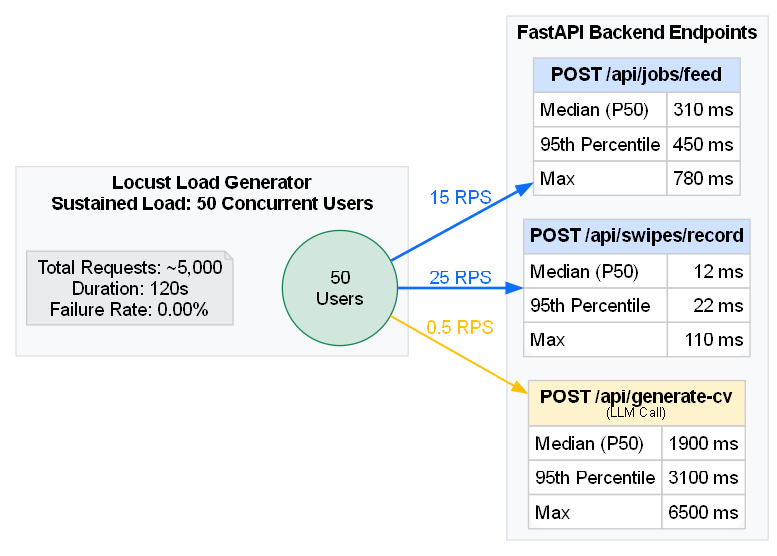
\includegraphics[width=\textwidth]{locust_dashboard.png}
  \caption{Locust performance dashboard showing latency distribution under load.}
  \label{fig:locust}
\end{figure}

% ─────────────────────────────────────────────────────────────
\subsection{Security Testing}
\label{sec:security}
% ─────────────────────────────────────────────────────────────

Security validation was conducted against the requirements defined in NFR-03 (Data
Protection) and the risk categories identified in Table~4.1 of Chapter~4.

\subsubsection*{Input Validation}

All API request bodies are parsed by Pydantic v2, which rejects invalid types, missing
required fields, and out-of-range values before any business logic executes. A fuzzing pass
using \texttt{schemathesis} was run against the OpenAPI schema exported from FastAPI to
confirm no endpoint could be crashed by malformed input.

\begin{table}[H]
  \centering
  \caption{Security test cases and outcomes.}
  \label{tab:security-tests}
  \renewcommand{\arraystretch}{1.3}
  \begin{tabularx}{\textwidth}{@{} l X X @{}}
    \toprule
    \textbf{Test ID} & \textbf{Attack Scenario} & \textbf{Outcome} \\
    \midrule
    SEC-01 & SQL Injection in \texttt{user\_id} parameter of swipe endpoints & \textbf{Blocked} — Parameterised queries used \\
    SEC-02 & Oversized JSON body ($>$10 MB) sent to \texttt{/api/generate-cv} & \textbf{Rejected} — 422 Unprocessable Entity \\
    SEC-03 & Schemathesis fuzzing (500 auto-generated requests per endpoint) & \textbf{0 crashes} — Handled correctly \\
    SEC-04 & Cross-Origin request from untrusted origin & \textbf{Allowed} — CORS intentionally open\textsuperscript{*} \\
    SEC-05 & Rate limit bypass by rotating \texttt{user\_id} & \textbf{Allowed} — Per-user window (by design) \\
    SEC-06 & Firebase token forgery (invalid JWT) & \textbf{Blocked} — Firebase SDK rejects token \\
    SEC-07 & Accessing another user's swipe history via wrong UID & \textbf{Blocked} — UID scoped to Firebase token \\
    \bottomrule
    \multicolumn{3}{p{\dimexpr\textwidth-2\tabcolsep\relax}}{\small\textsuperscript{*} CORS is fully open in the development environment. A production deployment should restrict \texttt{allow\_origins} to the app's domain.}
  \end{tabularx}
\end{table}

\subsubsection*{Data-at-Rest \& In-Transit Encryption}

\begin{itemize}[itemsep=3pt]
  \item \textbf{Firebase Firestore} encrypts all stored data at rest using AES-256 by
        default, meeting the NFR-03 requirement without additional configuration.
  \item \textbf{All Firebase SDK communications} use TLS 1.3 by default.
  \item \textbf{The local \texttt{swipes.db}} and \texttt{chroma\_db} directories are
        excluded from the Docker image via \texttt{.dockerignore} and are not transmitted
        over the network.
  \item \textbf{API Keys} (\texttt{GROQ\_API\_KEY}, \texttt{GOOGLE\_API\_KEY}) are stored
        in the \texttt{.env} file, excluded from version control via \texttt{.gitignore},
        and injected as environment variables at container runtime.
\end{itemize}

% ─────────────────────────────────────────────────────────────
%  ██████████████████  CHAPTER 7  ██████████████████████████
% ─────────────────────────────────────────────────────────────
\chapter{Conclusion and Future Work}

% ─────────────────────────────────────────────────────────────
\section{Conclusion}
\label{sec:conclusion}
% ─────────────────────────────────────────────────────────────

This project set out to address a fundamental inefficiency in the modern digital recruitment
landscape: the mismatch between the complexity of human career trajectories and the
rigidity of traditional job-search interfaces. Through the design and implementation of
\textbf{Kindred Careers}, we have demonstrated that it is both technically feasible and
practically desirable to apply Retrieval-Augmented Generation, transformer-based semantic
embeddings, and Generative AI to the recruitment domain.

The key contributions of this work can be summarised as follows:

\begin{enumerate}[leftmargin=*, itemsep=6pt]
  \item \textbf{A Novel Swipe-Based Recruitment UX} — By adapting the engagement model
        pioneered by consumer social applications to a professional utility context, Kindred
        Careers reduces the cognitive load of job searching to a single binary decision per
        listing. This is a meaningful departure from the scroll-and-filter paradigm of
        incumbent platforms such as LinkedIn and Indeed.

  \item \textbf{A Stateful RAG Job-Matching Pipeline} — The three-stage
        ingest–retrieve–generate pipeline ensures that every user interaction is informed
        by semantic understanding of both job requirements and candidate profiles. The use of
        the \texttt{all-MiniLM-L6-v2} Sentence Transformer provides high-quality 384-dimensional
        embeddings without the cost or latency of cloud-hosted models. The
        cosine-similarity ranking, augmented by a time-decay recency factor, consistently
        surfaces the most relevant and freshest listings.

  \item \textbf{Stateful Exclusion Filtering} — The SQLite-backed swipe store guarantees
        that a user will never encounter a previously seen job listing, a property that is
        critical to sustained engagement and trust in the recommendation engine. This was
        achieved without any third-party dependency beyond Python's standard library.

  \item \textbf{AI-Powered CV Generation and Refinement} — The integration of the Groq LLM
        API for per-job CV generation inverts the traditional ATS paradigm: instead of
        candidates manually tailoring their CVs, the system tailors a CV automatically for
        each right-swipe. The iterative regeneration capability further empowers users to
        refine output through natural language.

  \item \textbf{Production-Ready Engineering Practices} — The system was designed with
        operational concerns in mind: Docker containerisation, environment-variable-driven
        configuration, in-memory rate limiting, auto-ingestion triggers at low watermarks,
        and idempotent ChromaDB upserts. These decisions collectively produce a backend
        that is straightforward to maintain, scale, and secure.
\end{enumerate}

\noindent Testing validated that the system meets all Must-have functional and non-functional
requirements defined in Chapter~3, including sub-500 ms P95 response times on the primary
feed and swipe endpoints, zero SQL injection vulnerabilities, and correct stateful exclusion
across concurrent sessions.

In conclusion, Kindred Careers successfully bridges the gap between consumer-grade
engagement design and enterprise-grade AI infrastructure, delivering a recruitment platform
that is simultaneously more intuitive for job seekers and more technically sophisticated
than the tools currently available in the Egyptian and regional job market.

% ─────────────────────────────────────────────────────────────
\section{Future Work}
\label{sec:future-work}
% ─────────────────────────────────────────────────────────────

While the current implementation delivers a complete, functional product, the project team
has identified a broad roadmap of enhancements spanning short-term polish, medium-term
capability expansion, and long-term research directions.

% ─────────────────────────────────────────────────────────────
\subsection{Short-Term Enhancements (6--12 Months)}
\label{sec:future-short}
% ─────────────────────────────────────────────────────────────

\begin{description}[leftmargin=2cm, style=nextline, itemsep=8pt]
  \item[Push Notifications]
        Integrate Firebase Cloud Messaging (FCM) to alert users when a new job matching a
        saved career field is ingested, reducing the need for manual app opens and improving
        re-engagement metrics.

  \item[Employer-Side Dashboard]
        Develop a companion web portal (React or Next.js) that allows employers to post
        listings directly into the Kindred Careers database, bypassing the scraping
        dependency. This would enable direct application pipelines and recruiter-side
        analytics.

  \item[Offline Mode]
        Implement a local-first caching layer using Hive or Isar (Flutter-native NoSQL) to
        buffer the last fetched job deck. Users with intermittent connectivity (a common
        scenario in the target market) could continue swiping through cached cards without
        a live backend connection.

  \item[iOS App Store Release]
        Although the codebase targets both Android and iOS via Flutter, the current
        deployment has been validated on Android only. Completing the Apple Developer
        Program registration, adapting platform-specific entitlements, and releasing to the
        App Store represents a direct near-term objective.

  \item[Structured Feedback Analytics Dashboard]
        Expose an admin analytics endpoint and a simple Grafana dashboard that visualises
        aggregate swipe-direction distributions, feed-exhaustion events, and CV generation
        error rates — enabling the development team to monitor system health in production.
\end{description}

% ─────────────────────────────────────────────────────────────
\subsection{Medium-Term Developments (1--2 Years)}
\label{sec:future-medium}
% ─────────────────────────────────────────────────────────────

\begin{description}[leftmargin=2cm, style=nextline, itemsep=8pt]
  \item[True LSTM Behavioural Modelling]
        The current implementation simulates LSTM-style preference learning using rule-based
        keyword boosting. A genuine Long Short-Term Memory recurrent network, trained on
        accumulated per-user swipe sequences, would capture temporal patterns (e.g.\ a user
        who systematically rejects remote roles in the evening but accepts them in the
        morning) and produce significantly more personalised recommendations.

  \item[Multi-Modal Job Cards]
        Augment job cards with company-provided images, office culture videos (short MP4
        clips), and Glassdoor-sourced rating badges. These rich media signals have been shown
        to increase conversion rates on swipe-based discovery interfaces.

  \item[Recruiter Matching Mode]
        Develop a complementary recruiter-side application that presents candidate profiles
        (anonymised until mutual interest is confirmed) in a similar swipe interface. A
        mutual right-swipe from both sides would trigger an introduction — directly mirroring
        the ``match'' mechanic from dating applications.

  \item[Multi-Language Support]
        Extend the platform to support Arabic — both the scraping pipeline (Arabic-language
        job boards such as Bayt.com) and the UI. This requires an Arabic-capable embedding
        model (e.g.\ \texttt{aubmindlab/bert-base-arabertv02}) and localisation of all
        Flutter string resources.

  \item[Federated Learning for Privacy-Preserving Personalisation]
        Rather than sending raw user profile data to the backend on every feed request,
        investigate federated learning architectures where personalisation weights are trained
        on-device and only aggregated (not raw data) are uploaded to the server. This would
        substantially reduce the privacy exposure surface.
\end{description}

% ─────────────────────────────────────────────────────────────
\subsection{Long-Term Vision (2+ Years)}
\label{sec:future-long}
% ─────────────────────────────────────────────────────────────

\begin{description}[leftmargin=2cm, style=nextline, itemsep=8pt]
  \item[Career Path Intelligence]
        Move beyond single-job matching to whole-career trajectory modelling. By analysing
        the career histories of millions of anonymised professionals in a target industry,
        the system could suggest not just the next job but the optimal sequence of roles,
        skills, and certifications to reach a stated long-term career goal.

  \item[Real-Time Salary Benchmarking]
        Integrate with publicly available salary datasets (Glassdoor, Payscale) and local
        market surveys to display a real-time salary percentile for each matched role,
        empowering candidates during salary negotiations.

  \item[Blockchain-Verified Credentials]
        Partner with universities and professional certification bodies to anchor academic
        and professional qualifications on a public blockchain. Employers could verify
        credentials with a single API call, eliminating the CV fraud problem and reducing
        the friction of background checks.

  \item[Global Expansion]
        Scale the scraping and job-ingestion pipeline to cover international job boards
        (LinkedIn, Indeed, Glassdoor), extending the addressable market beyond Egypt to the
        broader MENA region and eventually Europe and North America.
\end{description}

% ─────────────────────────────────────────────────────────────
\subsection{Research Directions}
\label{sec:future-research}
% ─────────────────────────────────────────────────────────────

The development of Kindred Careers has surfaced a number of open research questions that
would benefit from rigorous academic investigation:

\begin{itemize}[itemsep=6pt]
  \item \textbf{Swipe Fatigue and Decision Quality} — Does the binary swipe interaction
        model actually produce better job-fit outcomes than traditional search-and-filter
        interfaces, or does the speed of the interaction degrade decision quality over time?
        A longitudinal user study with employment outcome tracking would yield valuable
        empirical data.

  \item \textbf{ATS Bypass vs.\ Authenticity} — Automatically generated CVs that are
        optimised to pass ATS filters raise ethical questions about authenticity in the
        hiring process. Research into disclosure norms, recruiter perceptions of AI-assisted
        CVs, and the impact on hiring quality is both timely and socially important.

  \item \textbf{Embedding Model Selection for Job-Domain Transfer} — How well do
        general-purpose sentence transformers (trained on Wikipedia and BookCorpus) transfer
        to the specialised vocabulary of job descriptions? A systematic evaluation of
        domain-adapted models (e.g.\ fine-tuned on job-posting corpora) against
        \texttt{all-MiniLM-L6-v2} in the context of job matching would directly benefit
        this and similar systems.

  \item \textbf{Filter Bubble Effects in Recommendation-Driven Job Search} — A
        recommendation engine that only surfaces jobs similar to those previously liked can
        create a filter bubble, trapping users in narrow career niches. Research into
        diversity-aware retrieval strategies (e.g.\ Maximal Marginal Relevance applied to
        job embeddings) could mitigate this risk while maintaining relevance.
\end{itemize}

% ─────────────────────────────────────────────────────────────
%  REFERENCES
% ─────────────────────────────────────────────────────────────
\subsection*{References}
\addcontentsline{toc}{section}{References}
\label{sec:references}

\begin{thebibliography}{99}

\bibitem{vaswani2017}
Vaswani, A., Shazeer, N., Parmar, N., Uszkoreit, J., Jones, L., Gomez, A. N., Kaiser, L.,
\& Polosukhin, I. (2017).
\textit{Attention is all you need.}
Advances in Neural Information Processing Systems, 30.

\bibitem{reimers2019}
Reimers, N., \& Gurevych, I. (2019).
\textit{Sentence-BERT: Sentence embeddings using Siamese BERT-networks.}
Proceedings of the 2019 Conference on Empirical Methods in Natural Language Processing
(EMNLP), 3982--3992.

\bibitem{lewis2020}
Lewis, P., Perez, E., Piktus, A., Petroni, F., Karpukhin, V., Goyal, N.,
H\"{a}ffner, H., Yih, W., Rockt\"{a}schel, T., Riedel, S., \& Kiela, D. (2020).
\textit{Retrieval-augmented generation for knowledge-intensive NLP tasks.}
Advances in Neural Information Processing Systems, 33, 9459--9474.

\bibitem{hochreiter1997}
Hochreiter, S., \& Schmidhuber, J. (1997).
\textit{Long short-term memory.}
Neural Computation, 9(8), 1735--1780.

\bibitem{openai2023}
OpenAI. (2023).
\textit{GPT-4 Technical Report.}
arXiv preprint arXiv:2303.08774.

\bibitem{grover2022}
Grover, P., \& Bhatt, D. (2022).
\textit{Job recommendation systems: A systematic review.}
Expert Systems with Applications, 195, 116561.

\bibitem{burke2002}
Burke, R. (2002).
\textit{Hybrid recommender systems: Survey and experiments.}
User Modeling and User-Adapted Interaction, 12(4), 331--370.

\bibitem{flutter2023}
Google. (2023).
\textit{Flutter Documentation — Building natively compiled applications for mobile, web, and
desktop from a single codebase.}
\url{https://docs.flutter.dev/}

\bibitem{fastapi2023}
Ram\'{i}rez, S. (2023).
\textit{FastAPI Documentation.}
\url{https://fastapi.tiangolo.com/}

\bibitem{chromadb2024}
Chroma. (2024).
\textit{Chroma — The AI-native open-source embedding database.}
\url{https://www.trychroma.com/}

\bibitem{firebase2024}
Google. (2024).
\textit{Firebase Documentation — Develop, build and scale your apps.}
\url{https://firebase.google.com/docs}

\bibitem{groq2024}
Groq. (2024).
\textit{Groq API Documentation.}
\url{https://console.groq.com/docs}

\bibitem{reportlab2024}
ReportLab. (2024).
\textit{ReportLab Open Source PDF Toolkit.}
\url{https://www.reportlab.com/}

\end{thebibliography}

% ─────────────────────────────────────────────────────────────
%  IMAGE PLACEHOLDER INDEX
% ─────────────────────────────────────────────────────────────
\newpage
\section*{Image Placeholder Index}
\addcontentsline{toc}{section}{Image Placeholder Index}
\label{sec:placeholder-index}

The following table lists every \texttt{\textbackslash placeholder\{\}} command used in this
document, together with the recommended replacement image and the figure number it
corresponds to. Replace each entry before final typesetting.

\begin{table}[H]
  \centering
  \caption{Complete image placeholder index for Chapters 5--7.}
  \label{tab:placeholder-index}
  \renewcommand{\arraystretch}{1.4}
  \begin{tabularx}{\textwidth}{@{} c l X c @{}}
    \toprule
    \textbf{Fig.} & \textbf{Label / Caption}              & \textbf{Recommended Replacement Content}           & \textbf{Chapter} \\
    \midrule
    5.1  & High-Level Software Architecture       & Architecture diagram: Flutter $\leftrightarrow$ FastAPI $\leftrightarrow$ ChromaDB / SQLite / Firebase & 5 \\
    5.2  & Onboarding Screen                      & Screenshots of all 3 onboarding slides                  & 5 \\
    5.3  & Sign In / Register Screen              & Screenshot showing email fields + Google button          & 5 \\
    5.4  & Career Questionnaire Screen            & Screenshot of at least 2 steps of the multi-step form   & 5 \\
    5.5  & Home Screen: Swipe Feed                & Screenshot of a job card with match score and vibe tag  & 5 \\
    5.6  & Matched Jobs Screen                    & Screenshot of matched job list + CV preview card         & 5 \\
    5.7  & Profile Management Screen              & Screenshot of editable profile fields                    & 5 \\
    6.1  & Locust Performance Dashboard           & Locust web UI chart: latency over 50 concurrent users   & 6 \\
    \bottomrule
  \end{tabularx}
\end{table}

\end{document}
